\documentclass[12pt]{ctexart}

\usepackage{mathtools}
\usepackage{geometry}
\geometry{a4paper}
\usepackage{graphicx} % 插入图片宏包
\usepackage{float} % 设置图片浮动位置的宏包
% \usepackage{subfigure} % 插入多图时用子图显示的宏包
\usepackage{isotope}
\usepackage{listings}
\usepackage{xcolor}
\usepackage{appendix}

\title{粒子输运理论基础第一次作业}
\author{汤松松 }
\date{2020.09.21}

\begin{document}

\maketitle
\section{\isotope[235]{U},\isotope[238]{U}的中子反应截面}
\isotope[235]{U},\isotope[238]{U}对于不同能量中子的吸收截面,鉴于低、中能区截面变化较大,故选择双对数坐标来绘制截面图;高能区选择线性坐标表示。能量分界点为1eV、100000eV。如图\ref{fig:U}可知,\isotope[235]{U}的截面比\isotope[238]{U}的截面大。
\begin{figure}[H]
    \centering
    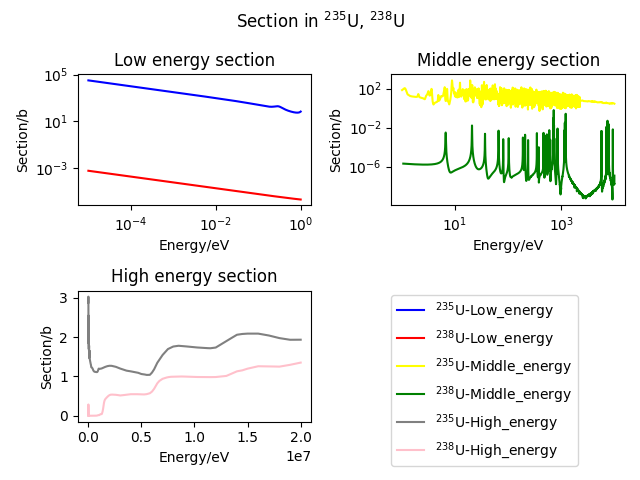
\includegraphics[width=0.9\textwidth]{img/Neutron section in U}
    \caption{Neutron section in U}
    \label{fig:U}
\end{figure}
\section{水($H_2O$)中的中子反应截面}
$H_2O$的反应截面如图\ref{fig:H2O},其中也包含\isotope[1]{H}和\isotope[16]{O}的反应截面。并且将不平滑区域($E > 10^5\ {\rm eV}$)的截面单独绘制。
\begin{figure}[H]
    \centering
    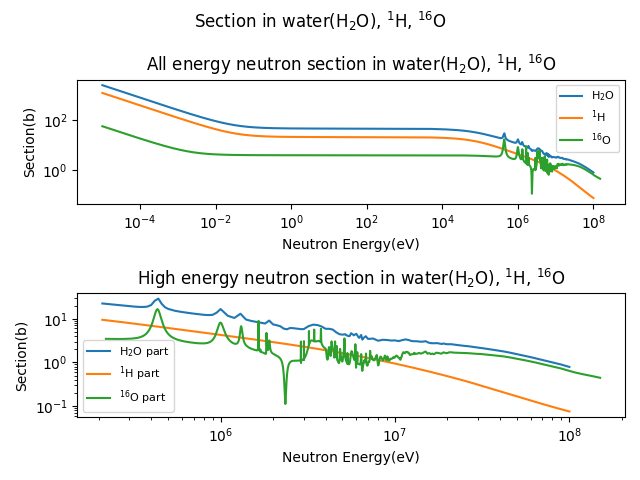
\includegraphics[width=0.9\textwidth]{img/Neutron section in water}
    \caption{Neutron section in water($H_2O$)}
    \label{fig:H2O}
\end{figure}

\begin{appendices}
\section{Python代码}
\lstinputlisting[language = Python]{barn_plot.py}
\end{appendices}

\end{document}